
%(BEGIN_QUESTION)
% Copyright 2010, Tony R. Kuphaldt, released under the Creative Commons Attribution License (v 1.0)
% This means you may do almost anything with this work of mine, so long as you give me proper credit

This high-temperature shutdown sensor uses a {\it thermistor} to sense temperature.  The thermistor has a negative temperature coefficient (i.e. resistance decreases as temperature increases):

$$\includegraphics[width=15.5cm]{i04746x01.eps}$$

Your task is to figure out how to ``trip'' this high-temperature alarm to test its operation, by ``tricking'' the relay module to think the thermistor is at a dangerously high temperature when in fact it is not.  In other words, you must devise an ``in-place'' test for the switch that may be performed at any time, even with the thermistor still sensing real process temperature.  Feel free to sketch your solution on the schematic diagram if it helps.

\underbar{file i04746}
%(END_QUESTION)





%(BEGIN_ANSWER)

{\it Any electrical modification to temporarily reduce the voltage drop between terminals 2 and 3 will work, and is worth full credit.  This includes:}

\begin{itemize}
\item{} Disconnecting wire to terminal 1 (at either terminal block)
\item{} Shorting terminals 2 and 3 (at either terminal block)
\end{itemize}

{\it Award half-credit for answers such as:}

\begin{itemize}
\item{} Break 2.7 k$\Omega$ resistor in half
\item{} Any potentiometer solution where returning to regular operation means having to set it at some mid-position value where the calibration is likely to be adversely affected
\end{itemize}

%(END_ANSWER)





%(BEGIN_NOTES)

{\bf This question is intended for exams only and not worksheets!}

%(END_NOTES)


